\begin{figure}[H]
\centering
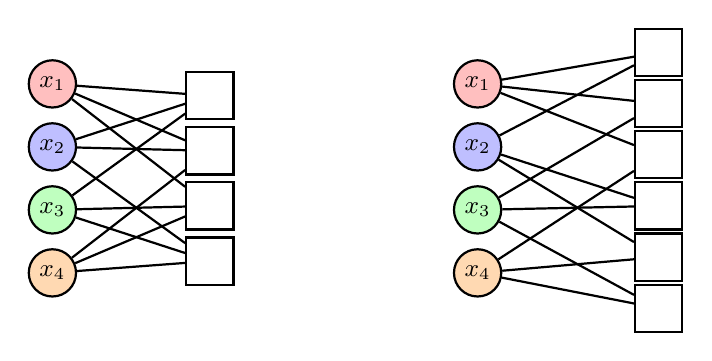
\begin{tikzpicture}[
    font=\small,
    % variable colors (consistent with previous figures)
    v1/.style={circle, draw, thick, fill=red!25,    minimum size=6mm, inner sep=0pt},
    v2/.style={circle, draw, thick, fill=blue!25,   minimum size=6mm, inner sep=0pt},
    v3/.style={circle, draw, thick, fill=green!25,  minimum size=6mm, inner sep=0pt},
    v4/.style={circle, draw, thick, fill=orange!30, minimum size=6mm, inner sep=0pt},
    fac/.style={rectangle, draw, thick, minimum width=6mm, minimum height=6mm, inner sep=0pt},
    edge/.style={draw, thick},
]

% =========================================================
% Left panel: 4 factors of arity 3
% =========================================================
\begin{scope}[shift={(0,0)}]
% variables (left column)
\node[v1] (v1L) at (0,  1.2) {$x_1$};
\node[v2] (v2L) at (0,  0.4) {$x_2$};
\node[v3] (v3L) at (0, -0.4) {$x_3$};
\node[v4] (v4L) at (0, -1.2) {$x_4$};

% factors (right column)
\node[fac] (f123) at (2.0,  1.05) {};
\node[fac] (f124) at (2.0,  0.35) {};
\node[fac] (f134) at (2.0, -0.35) {};
\node[fac] (f234) at (2.0, -1.05) {};

% edges (each arity-3 factor connects to its three variables)
\draw[edge] (v1L) -- (f123);
\draw[edge] (v2L) -- (f123);
\draw[edge] (v3L) -- (f123);

\draw[edge] (v1L) -- (f124);
\draw[edge] (v2L) -- (f124);
\draw[edge] (v4L) -- (f124);

\draw[edge] (v1L) -- (f134);
\draw[edge] (v3L) -- (f134);
\draw[edge] (v4L) -- (f134);

\draw[edge] (v2L) -- (f234);
\draw[edge] (v3L) -- (f234);
\draw[edge] (v4L) -- (f234);

%\node[align=center] at (1.0, 1.9) {Approximation with\\four arity-$3$ factors};
\end{scope}

% =========================================================
% Right panel: 6 factors of arity 2 (stacked with extra padding)
% =========================================================
\begin{scope}[shift={(5.4,0)}]
% variables (left column)
\node[v1] (v1R) at (0,  1.2) {$x_1$};
\node[v2] (v2R) at (0,  0.4) {$x_2$};
\node[v3] (v3R) at (0, -0.4) {$x_3$};
\node[v4] (v4R) at (0, -1.2) {$x_4$};

% factors stacked on the right (increased vertical spacing)
% spacing here is 0.65 between consecutive factor nodes
\node[fac] (f12) at (2.3,  1.60) {};
\node[fac] (f13) at (2.3,  0.95) {};
\node[fac] (f14) at (2.3,  0.30) {};
\node[fac] (f23) at (2.3, -0.35) {};
\node[fac] (f24) at (2.3, -1.00) {};
\node[fac] (f34) at (2.3, -1.65) {};

% edges (each factor connects to its two variables)
\draw[edge] (v1R) -- (f12);
\draw[edge] (v2R) -- (f12);

\draw[edge] (v1R) -- (f13);
\draw[edge] (v3R) -- (f13);

\draw[edge] (v1R) -- (f14);
\draw[edge] (v4R) -- (f14);

\draw[edge] (v2R) -- (f23);
\draw[edge] (v3R) -- (f23);

\draw[edge] (v2R) -- (f24);
\draw[edge] (v4R) -- (f24);

\draw[edge] (v3R) -- (f34);
\draw[edge] (v4R) -- (f34);

%\node[align=center] at (1.15, 1.9) {Approximation with\\six arity-$2$ factors};
\end{scope}

\end{tikzpicture}
\caption{Factor-graph view of arity control for posterior approximations.
Left: an approximation using four factors of arity $3$ (one per triple subset of variables).
Right: an approximation using six pairwise factors (one per variable pair).}
\label{fig:chapter_5_controlled_graph_arity_factorgraph}
\end{figure}
